\section{Research Plan}

Experiments will be conducted using the HyperNEAT (Hypercube based Neuroevolution of Augmenting Topologies) indirect encoding and the FT-NEAT (Fixed Topology NEAT) direct encoding for neural networks, a standard choice in the field \cite{Stanley2009ANetworks,Clune2011OnRegularity}. Length of evolutionary trials (2500 generations), fitness-based selection parameters, population size, and other parameters relating to the evolutionary process will be chosen in accordance with \cite{Clune2011OnRegularity}. The experiment will be performed in three problem domains that allow for ready, and well-understood, manipulation of problem regularity: the target weights problem, the bit mirroring problem, and the Quadruped controller problem \cite{Clune2011OnRegularity}. 

In the control experiment, the fitness score of each individual will be computed as the raw performance of that individual in the problem domain. In other trials, variants of an individual will be generated via mutations of the direct representation of the individual. For each trial, three runs will be conducted in which the fitness of each individual will be computed from the performances of 200 variants of that individual at one of three quartiles: the 50th, 75th, or 100th. Adjustments to problem regularity and mutation severity will also be evaluated for each trial. While generating and testing a large number of variants of each individual is computationally expensive, this approach is highly paralellizable and feasible with the computing resources available to academic research groups \cite{Mengistu2016EvolvabilityIt}.

\begin{figure}
 \centering
    \begin{subfigure}[b]{0.5\textwidth}
        \centering
    	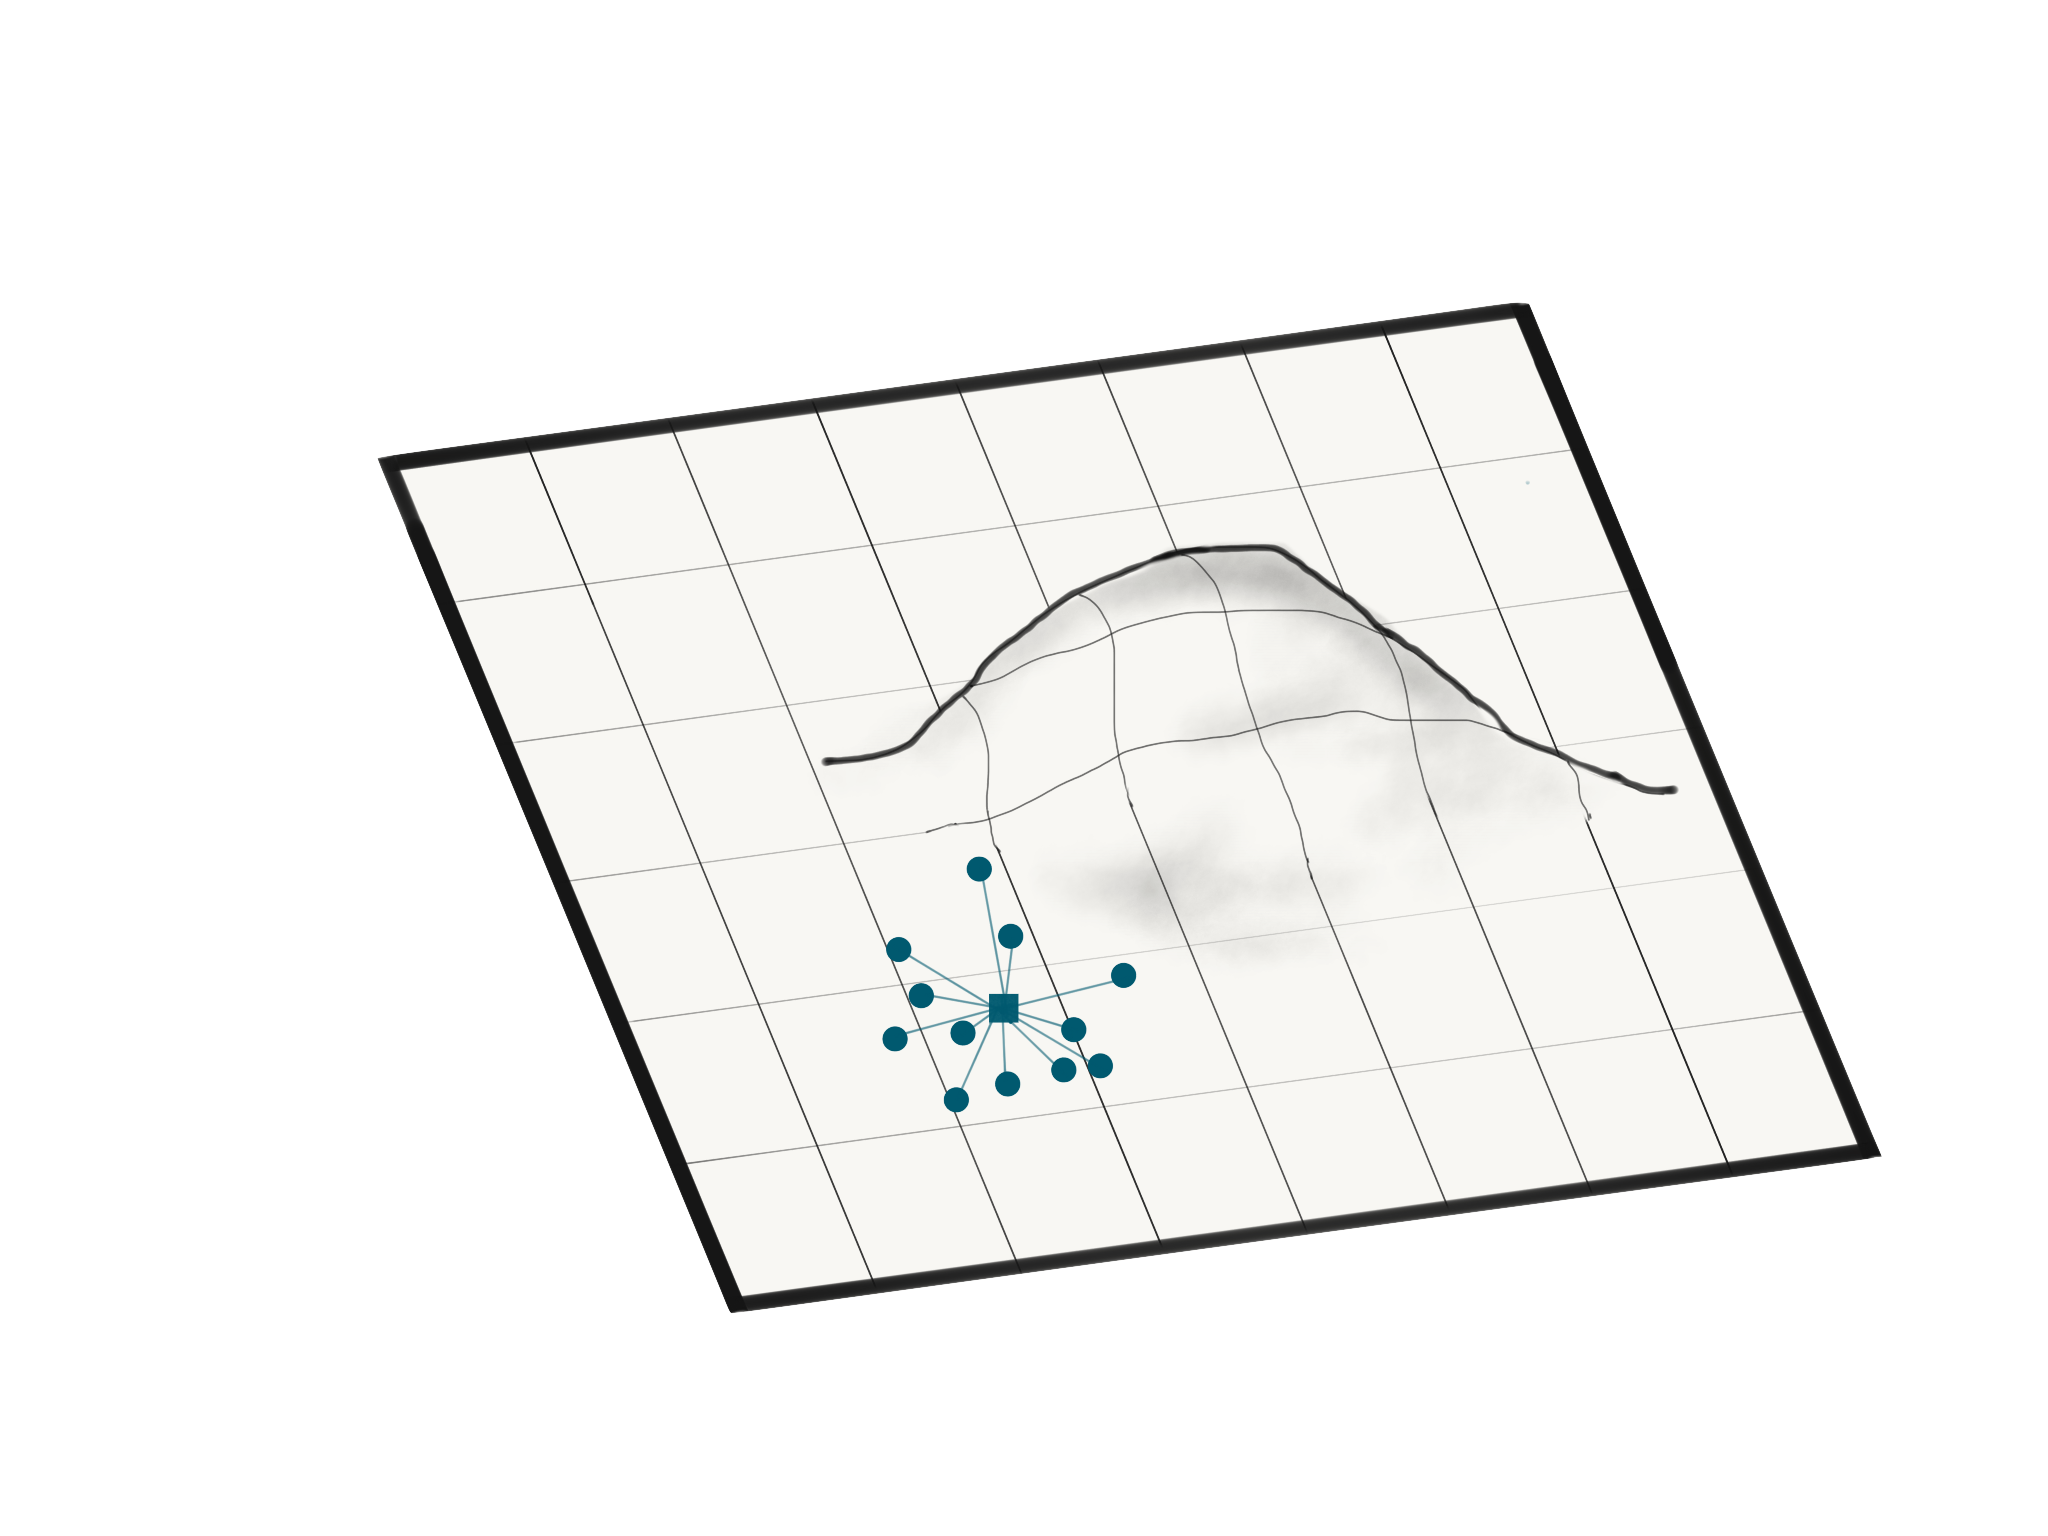
\includegraphics[width=\textwidth]{img/static_mutation.png}
        \caption{direct mutation}
        \label{subfig:static_mutation}
    \end{subfigure}%
    \hfill
    \begin{subfigure}[b]{0.5\textwidth}
        \centering
        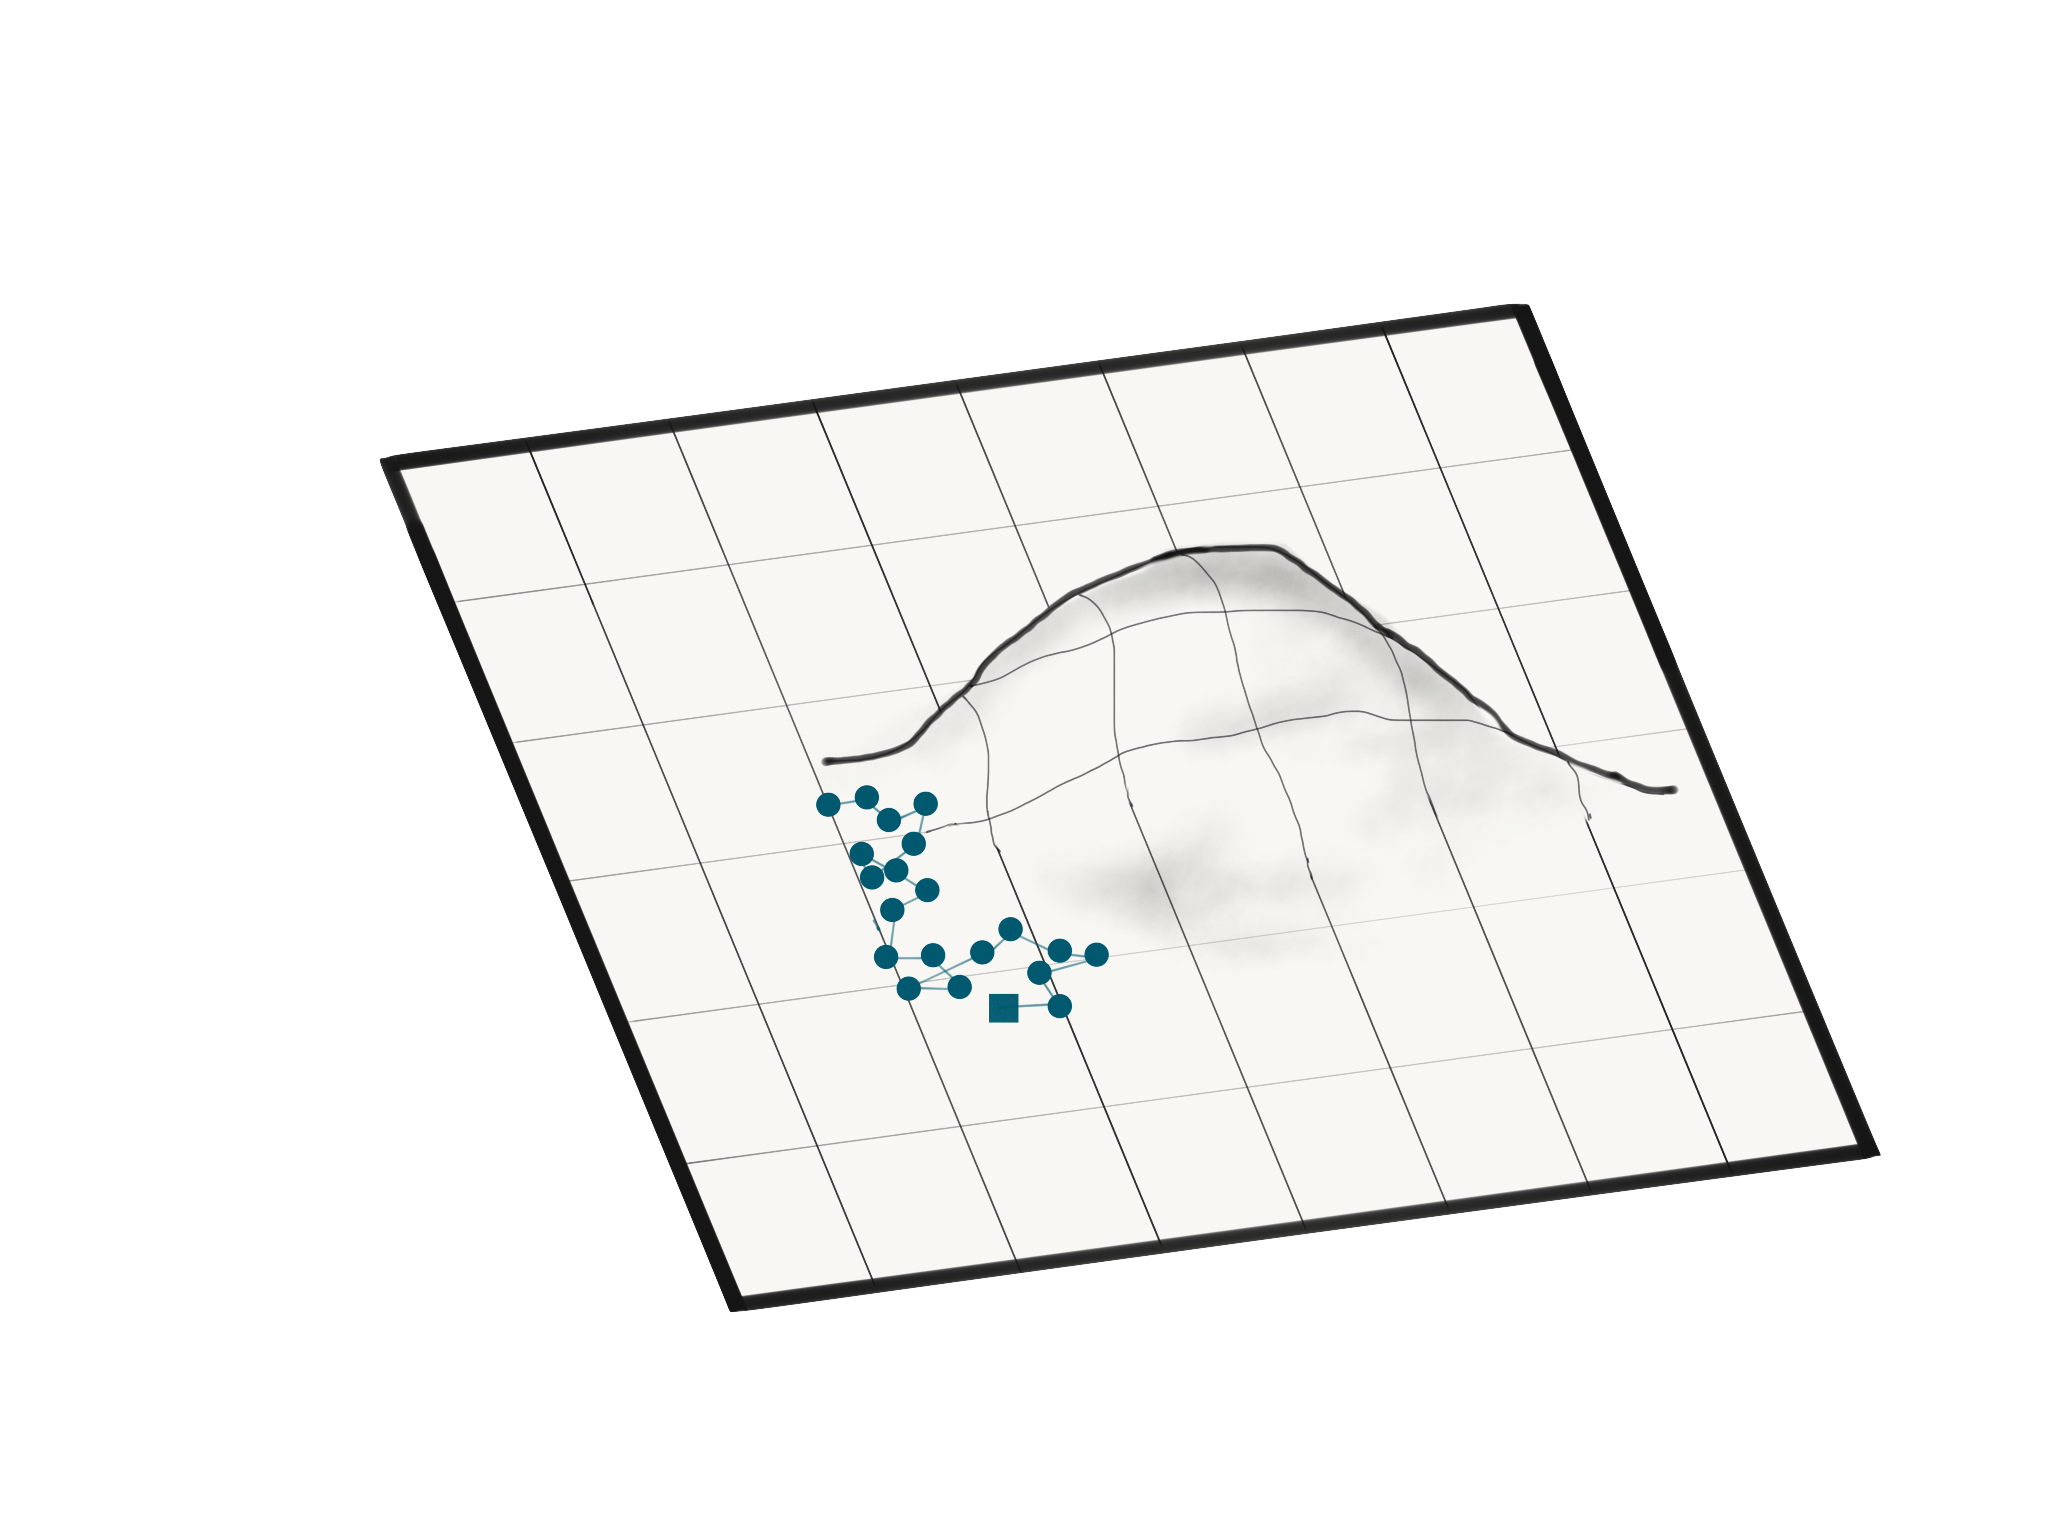
\includegraphics[width=\textwidth]{img/random_walk.png}
        \caption{random walk}
        \label{subfig:random_walk}
    \end{subfigure}
    \hfill
    \begin{subfigure}[b]{0.5\textwidth}
        \centering
        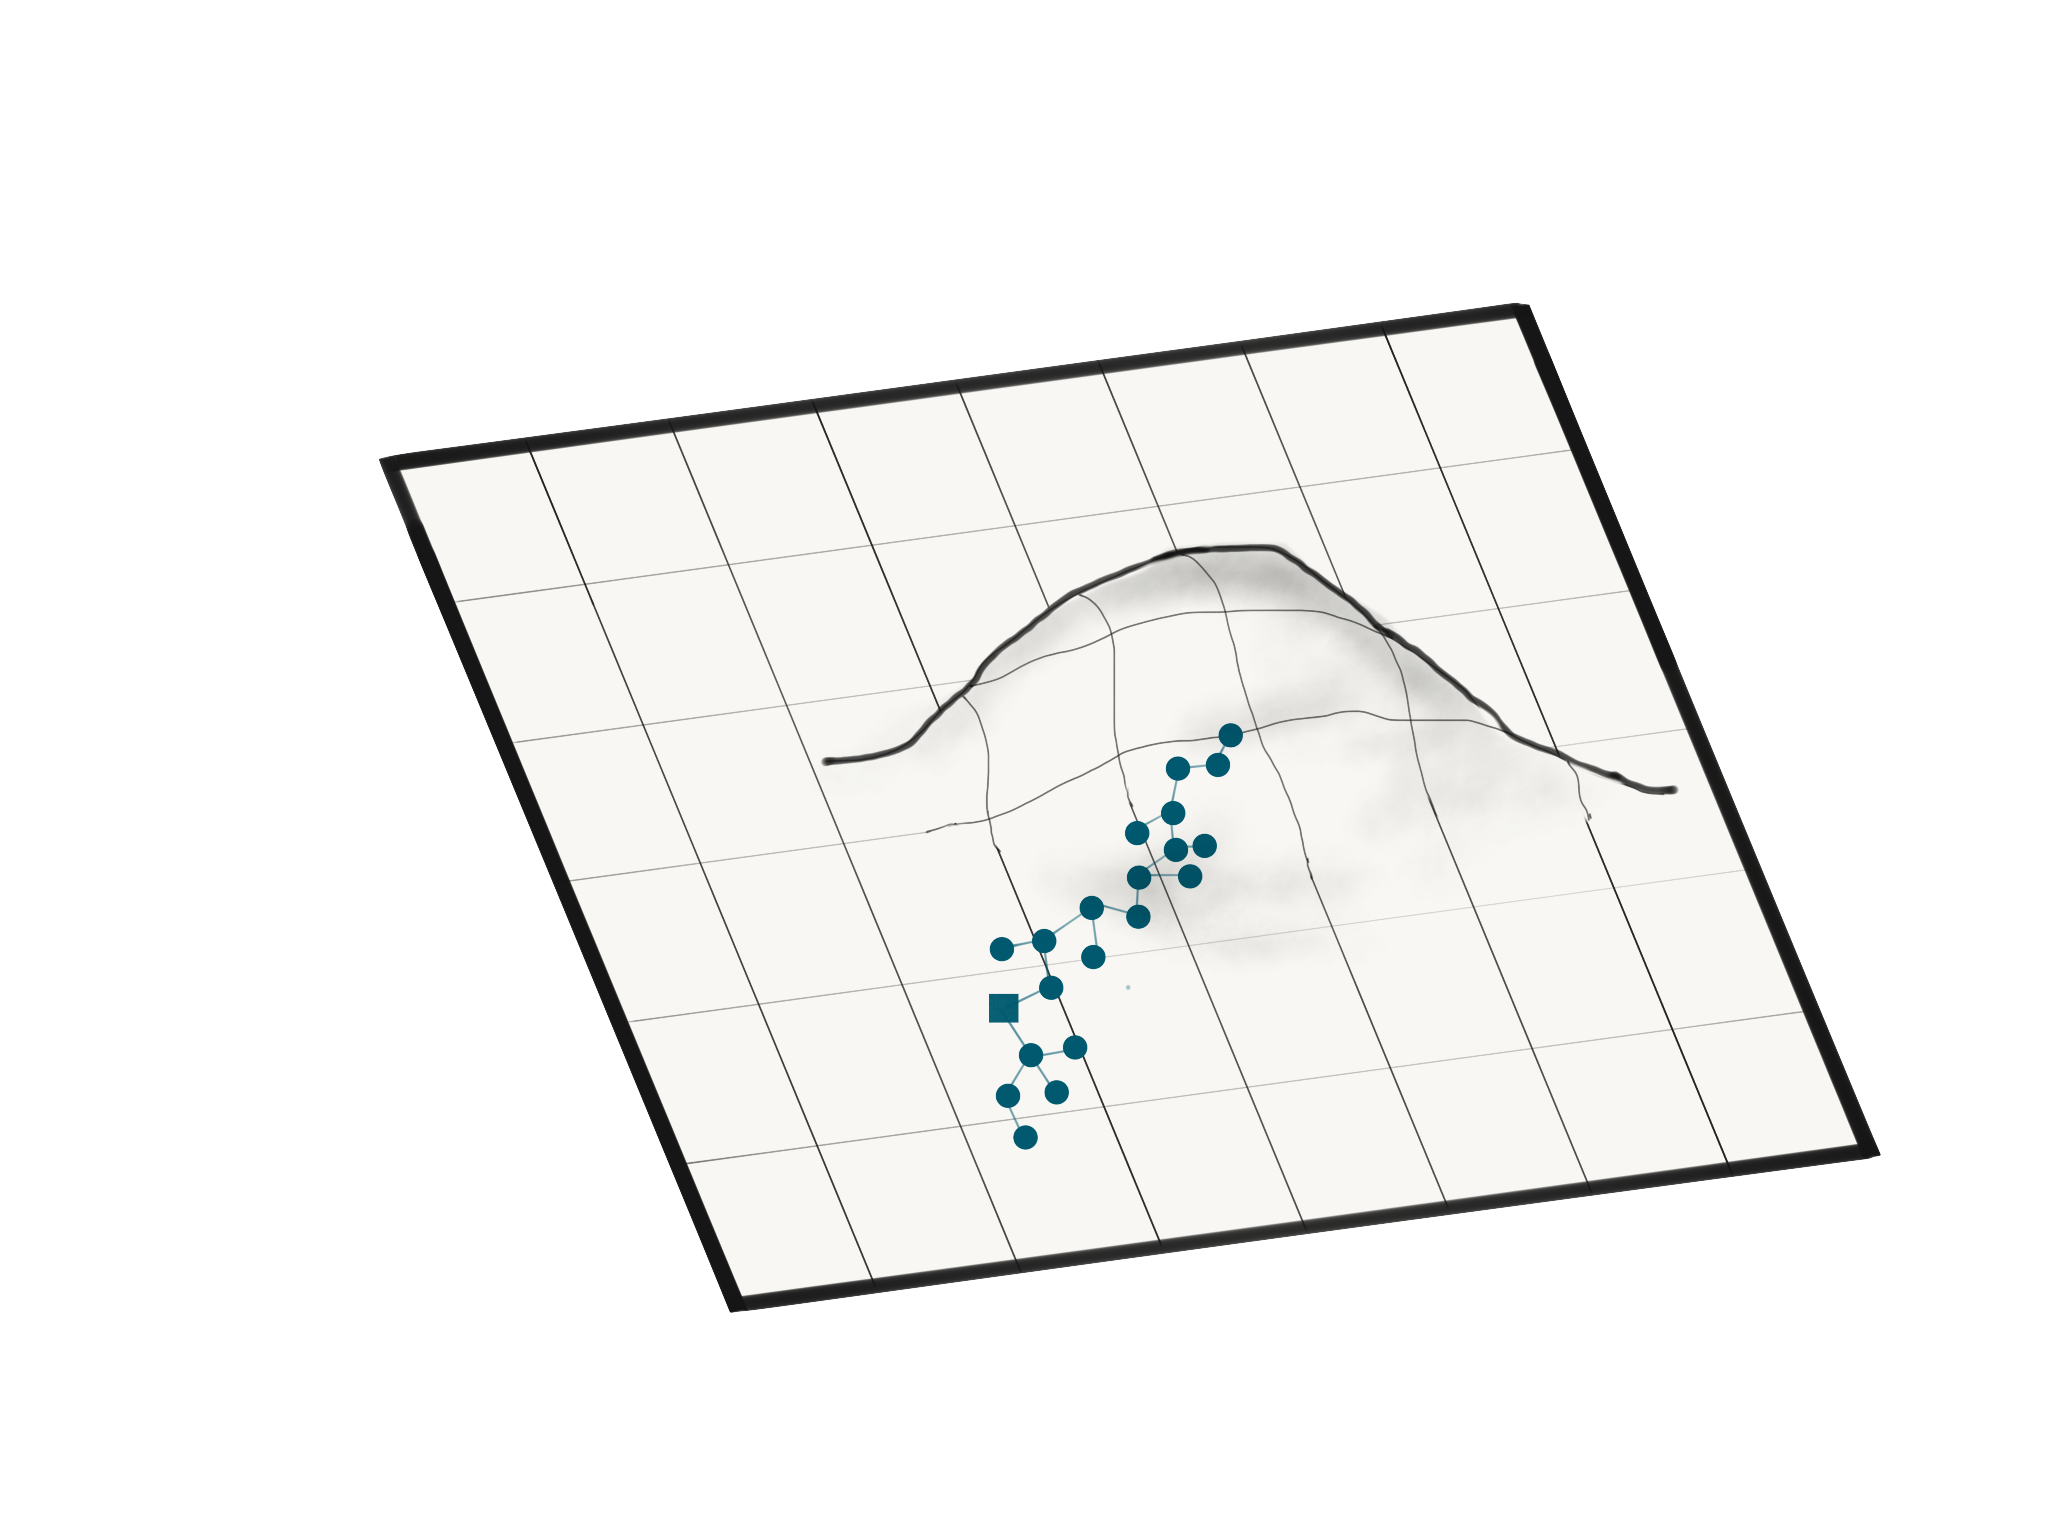
\includegraphics[width=\textwidth]{img/simulated_annealing.png}
        \caption{simulated annealing}
        \label{subfig:simulated_annealing}
    \end{subfigure}
 	\captionsetup{singlelinecheck=off,justification=raggedright}
    \vspace{-2ex}
  \captionsetup{singlelinecheck=off,justification=raggedright}
  \caption{The three modes of local phenotype space search proposed are illustrated. In each illustration, the phenotype space is depicted as a three dimensional surface with points on the surface representing different phenotypes and the height of the surface denoting the fitness of the phenotypes at those points. The original phenotype mapped to by a genetic representation is shown with a square. Points marked with a circle denote phenotypes explored during the local search processes. Lines connecting the points represent that one point was reached from the other by a mutation of the direct representation of a phenotype. Subfigure \ref{subfig:static_mutation} depicts the direct mutation local phenotypic search process, where points explored are generated by mutations to the direct representation of the original phenotype mapped to by a genetic representation. Subfigure \ref{subfig:random_walk} depicts the random walk local phenotypic search process, where points explored are generated by mutation to the direct representation of the point explored immediately before (starting from the direct representation of the original phenotype mapped to by a genetic representation). Finally, subfigure \ref{subfig:simulated_annealing} depicts the simulated annealing local phenotypic search process, where points are explored via mutation to the direct representation of a randomly chosen point previously explored with an increasingly strong bias towards exploring from points with high fitness as the exploration process proceeds.}
  \label{fig:local_search_types}
\end{figure}

In the first naive developmental variance trial, variants will be generated from mutations stemming from the direct representation of that individual (Figure \ref{subfig:static_mutation}). In the second naive developmental variance trial, variants will be generated from ten mutational random walks that emanate from the direct representation of the individual (Figure \ref{subfig:random_walk}). Finally, in the third developmental variance trial, variants will be generated by a simulated-annealing search of the local phenotypic space surrounding the individual guided by the distribution of fitness scores across that space (Figure \ref{subfig:simulated_annealing}). 

After 2500 generations of evolution operating on the HyperNEAT indirect genetic representation of networks, all populations will be switched over to direct representations (FT-NEAT) and the evolutionary process run for another 2500 generations (using direct evaluation of and individual's performance as the fitness metric) \cite{Clune2011OnRegularity}. All trials will be evaluated using the maximum performance of the unaltered phenotype of individuals at the end of the HyperNEAT evolutionary stage, the maximum performance of individuals at the end of the FT-NEAT evolutionary stage, and the amount of fitness gained during the FT-NEAT evolutionary stage.


% At each individual fitness evaluation, a set of alternate phenotypes will be generated from the phenotype generated by HyperNEAT by translating it to a direct encoding and then applying mutations to the direct encoding. This would . Trials will be conducted where the phenotypic variants are generated by a directed simulated-annealing hill-climbing search of the local mutation space directed by the fitness score of individuals, a random walk through the phenotype space, and mutations stemming from the original phenotype. Fitness scores will be generated from these collections phenotypic variants via maximum, mean, and median

% As in \cite{Mengistu2016EvolvabilityIt}, 

% In the first part of the project, irregularization via direct encoding would be considered. The biological analogy for this would be environmental influence on the phenotype. . . . We would be testing to see what the fitness performance reached by hyperNEAT before FT-NEAT is, how much FT-NEAT is able to improve that fitness performance, and what the ultimate fitness of the whole hbyrID process. The exact parameters used in the simulation would be chosen based on the example set by \cite{clune2011OnRegularity} and via trial and error, as is standard practice.

% \begin{itemize}
%   \item 
%   \item Monte Carlo sample of phenotypic space surrounding individual: undirected search/directed/learning search; mean/median/maximum
%   \item after, try irregularizing with direct encoding further evolution (i.e. FT-NEAT) or by evolving/applying local learning rules
%   \item idea: use hyperNEAT to indirectly encode learning rules \cite{Risi2010IndirectlyRules}
%   \item 
% \end{itemize}